\section{Multi-Layer Perceptrons}

\subsection{Model}

In this part, we implemented a simple multi-layer perceptron network.

We trained the network with the Adam optimizer, and the ReLU activation function was used on all hidden layers.
The batch size was set to $184$, i.e. the whole dataset.

Similar to previous sections, we combined it with grid search and optimized a number of hyper-parameters through cross-validation within the training dataset. We optimized for the following:

\begin{enumerate}[a.]
    \item Architecture. We tried a number of architectures, from smaller single hidden layers (size 8) to multiple bigger layers (size 32). For us the best performing architecture in our setup was a single layer of size 26.
    \item L2 regularization term $\alpha$. We used the L2 regularization (as opposed to L1) because it shrinks feature coefficients evenly and so works better for features that might be codependent. We tried a number of coefficients between $0.1$ and $10$ and achieved the best performance with $\alpha \approx 0.32$.
    \item Learning rate. Out of several values, the best performing was $0.0001$.
    \item The number of epochs was set to 1000, which proved to be enough, while more epochs did not lead to better performance.
\end{enumerate}

\begin{figure}
    \centering
    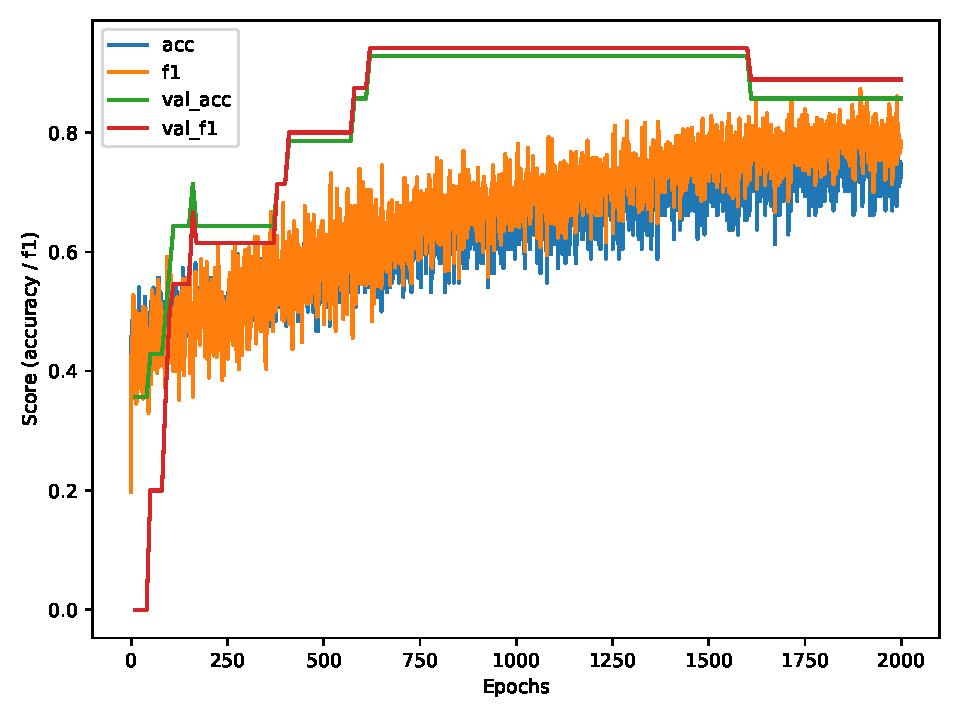
\includegraphics[width=1\columnwidth]{images/mlp_training.pdf}
    \caption{A plot of the training history of the multi-layer perception. On the same axis are the F1 measure and accuracy for comparison. This model was trained only on $90\%$ of the training data to allow the $10\%$ data for validation during training for vizualization purposes. Metrics on the validation data were evaluated every $10$ epochs.}
    \label{fig:mlp_training}
\end{figure}

We also used the dropout value of 0.8, which allowed the model to generalize better, improving the F1 score on the test dataset. \autoref{fig:mlp_training} shows the training history of the MLP. The final model trained on the whole training dataset achieves the F1 score of $0.8$ on the test dataset.

\subsection{Explaining predictions}

In this section, we explain how each feature contributes to predictions of the MLP model. We do so using the SHAP framework \cite{lundbergUnifiedApproachInterpreting2017}.

Of the various explainer algorithms offered by the SHAP Python library, we used the \texttt{Exact} explainer. It is model-agnostic, which fits our use case, and precise since this algorithm does not approximate the result by subsampling. The major disadvantage is the exponential complexity of computing Shapley values in the number of features; however, the computation time is, in practice, feasible for the use case of this project.

We give the explainer as the input the pre-trained MLP model, and the training dataset, which is to be used for masking out feature values during Shapley values calculations. We then feed in the test dataset, on which the Shapley values are calculated.

\begin{figure}
    \centering
    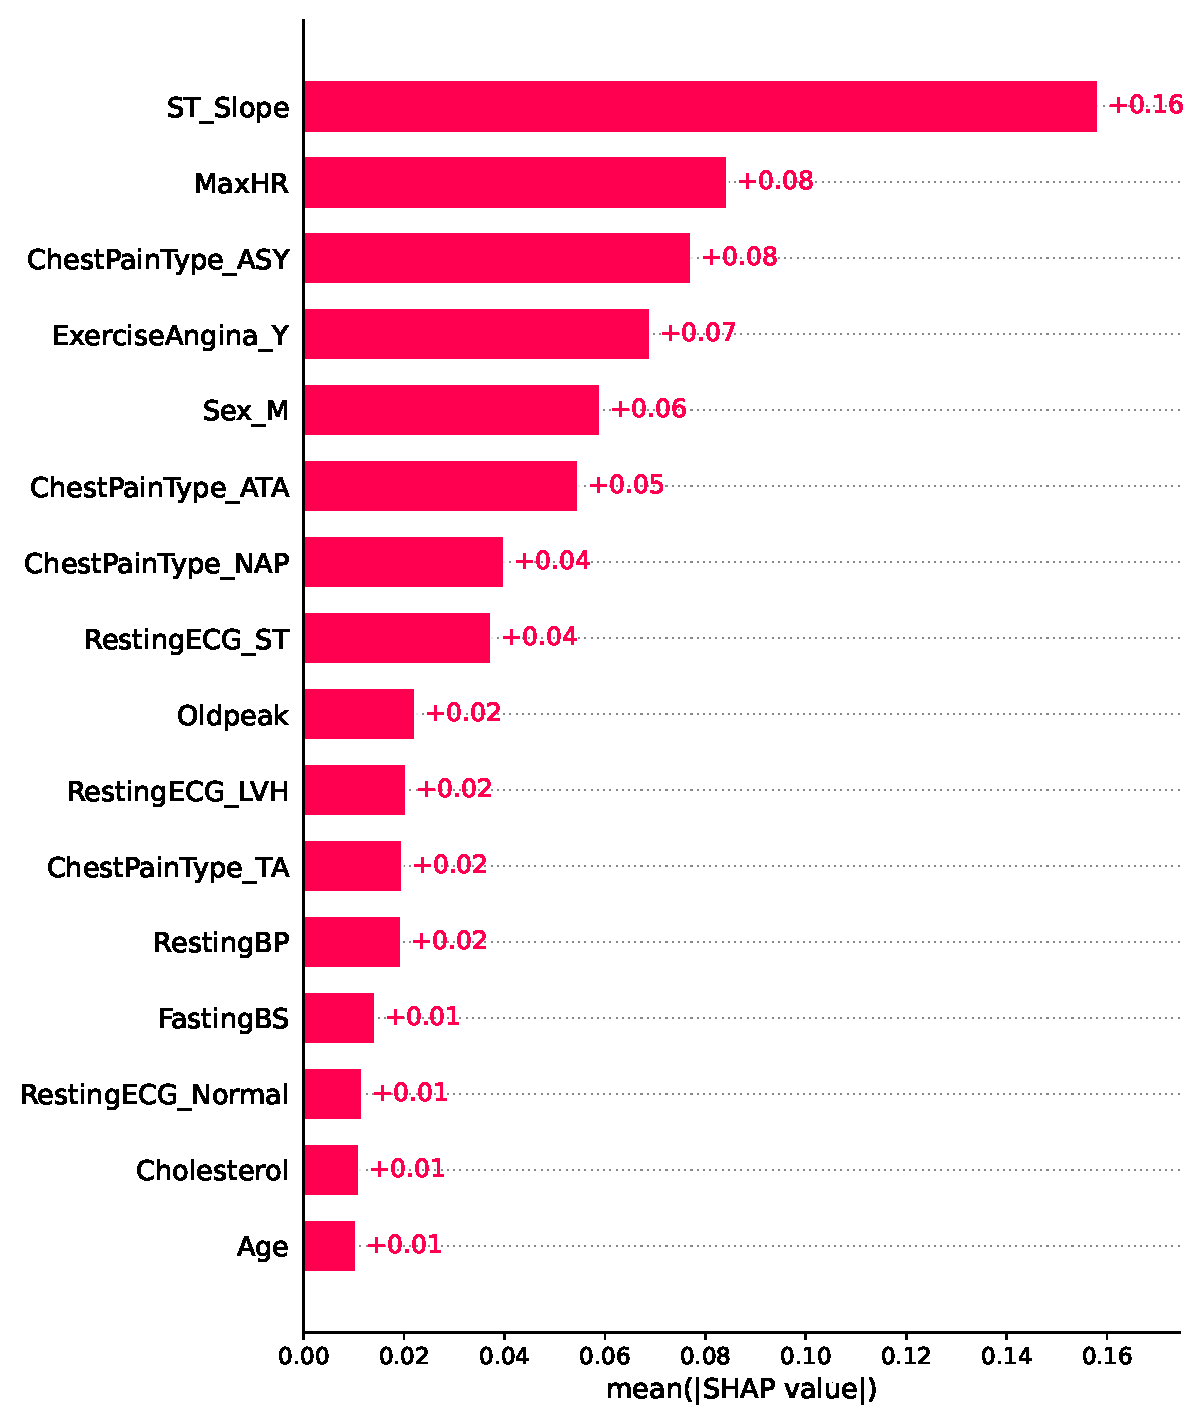
\includegraphics[width=0.8\columnwidth]{images/shap_bar.pdf}
    \caption{Bar vizualization of feature importances of the overall MLP model, averaged on the test dataset.}
    \label{fig:shap_bar}
\end{figure}
\begin{figure}
    \centering
    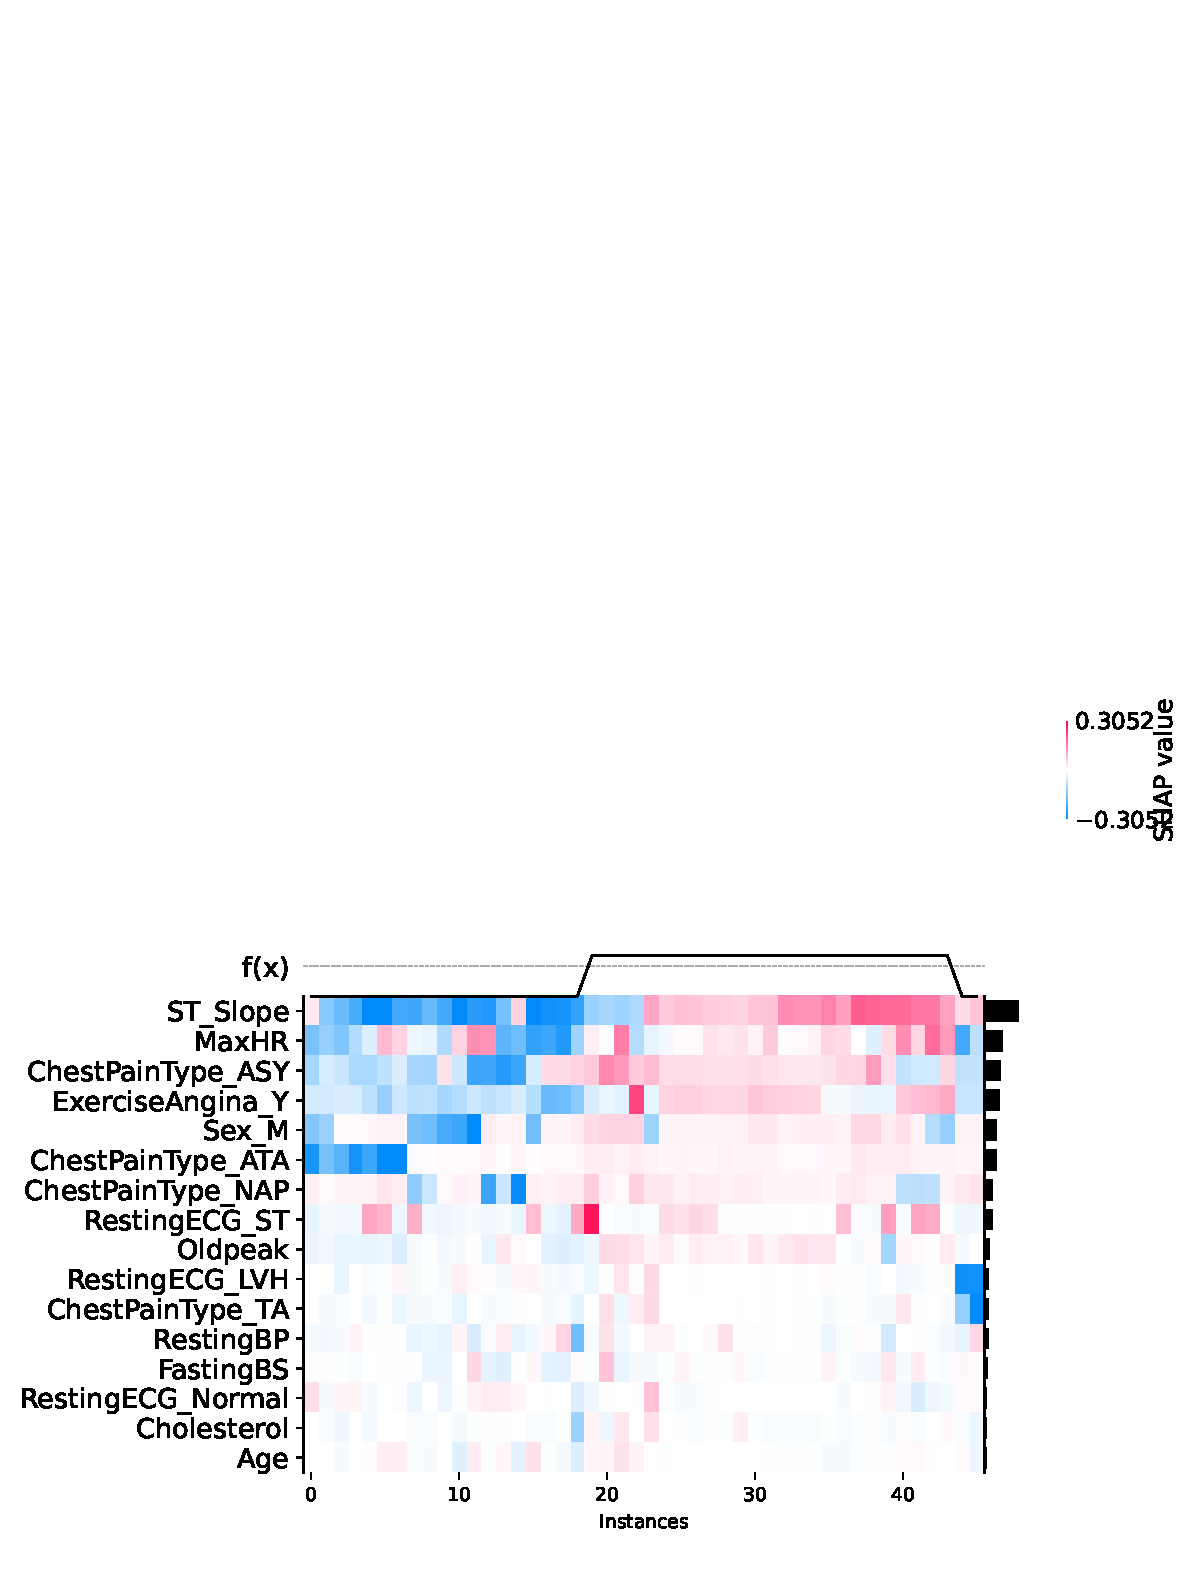
\includegraphics[trim=0 0 2.8cm 16cm,clip,width=1\columnwidth]{images/shap_heatmap.pdf}
    \caption{Heatmap vizualization of per-sample feature importance of the MLP model, on the test dataset. Each cell's color corresponds to the amount the feature (row) influences the prediction of the sample (column). Columns are ordered by hierarchical clustering of the samples. The bars on the right show overall feature importance across the test dataset.}
    \label{fig:shap_heatmap}
\end{figure}
\begin{figure}
    \centering
    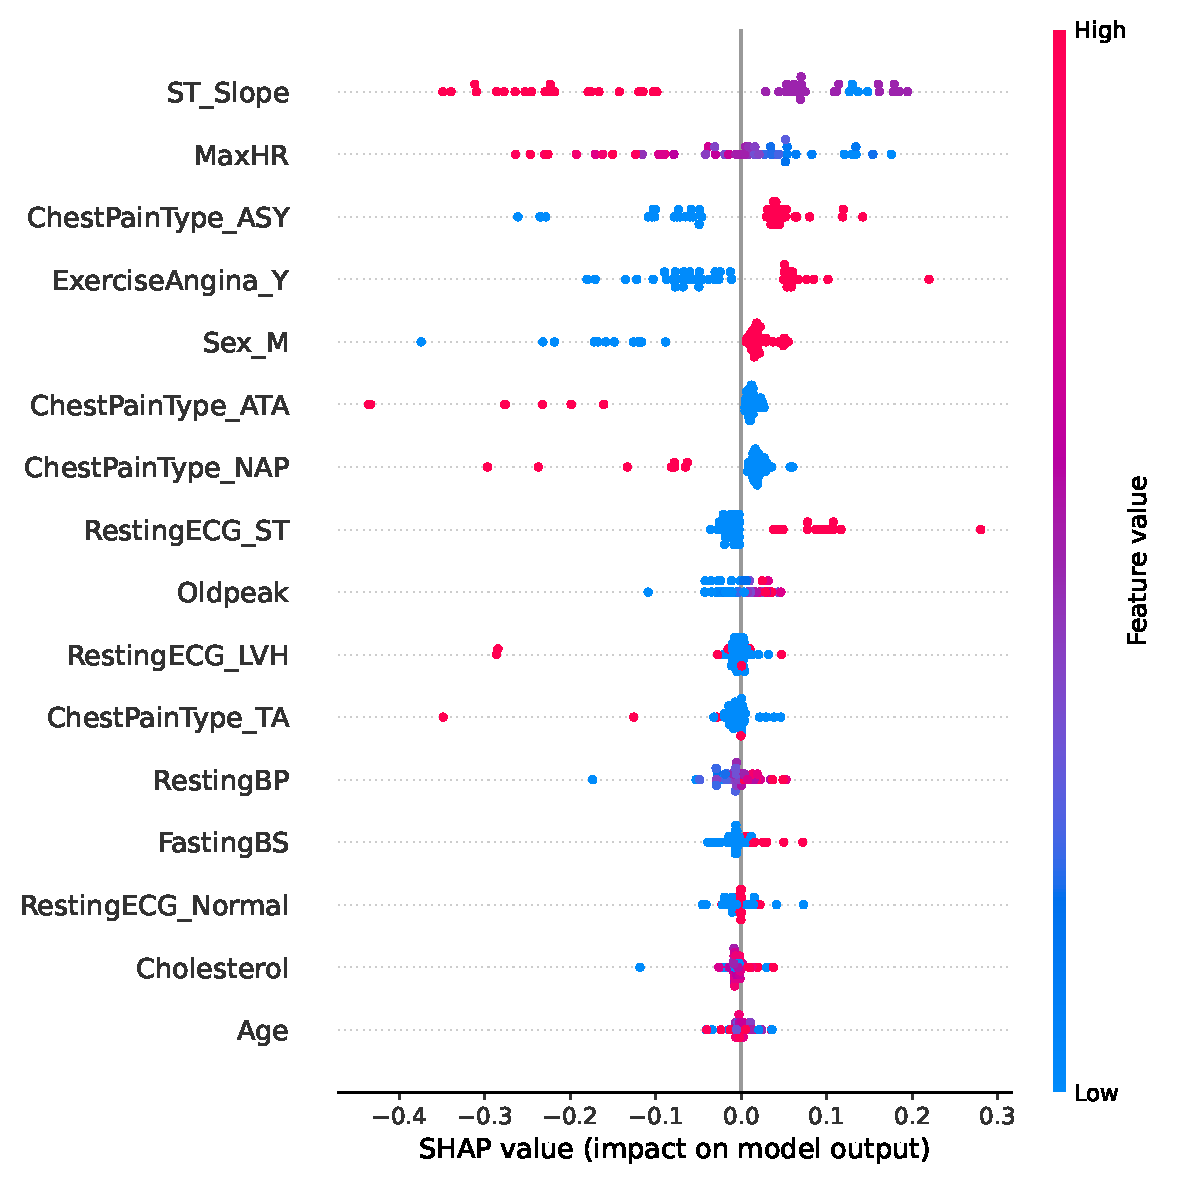
\includegraphics[width=1\columnwidth]{images/shap_beeswarm.pdf}
    \caption{Beeswarm vizualization of feature importances of the overall MLP model on the test dataset. Each marker corresponds to a sample in the test dataset.}
    \label{fig:shap_beeswarm}
\end{figure}
\begin{figure}
    \centering
    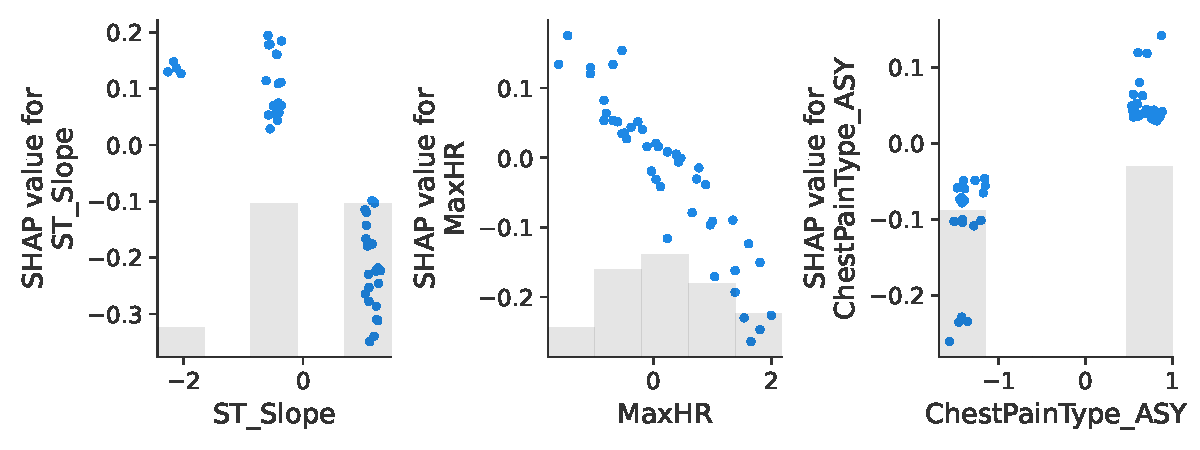
\includegraphics[width=1\columnwidth]{images/shap_scatter.pdf}
    \caption{Scatter plot vizualization of the three most important features according to our SHAP analysis. Individual points correspond to samples in the test dataset. The x-axis is the feature value, and the y-axis is the feature's relative contribution to the final prediction of the sample.}
    \label{fig:shap_scatter}
\end{figure}

\Cref{fig:shap_bar,fig:shap_heatmap,fig:shap_beeswarm} vizualize overall feature importances on the test dataset, using bar (\autoref{fig:shap_bar}), heatmap (\autoref{fig:shap_heatmap}), and beeswarm (\autoref{fig:shap_beeswarm}) plots. \Cref{fig:shap_sample_positive,fig:shap_sample_negative} explain the predictions of four positive and negative samples, respectively.

We note that for the correctly predicted samples, the sets of highly influential features are similar to those identified as important in Q2. Namely, \texttt{ST\_Slope} and \texttt{MaxHR} are each among the top 3 most important features in $5$ out of $6$ correctly predicted samples in \cref{fig:shap_sample_positive,fig:shap_sample_negative}; and \texttt{ChestPainType\_ASY} is among the top $5$ features in $5$ out of $6$ correct predictions. \autoref{fig:shap_scatter} shows a scatter plot of the influence of the three most important features by SHAP.

The features \texttt{Age} and \texttt{RestingBP} which were identified as relatively important according to the Gini importance in Q3, are identified as unimportant according to SHAP (\autoref{fig:shap_bar}).

Further, we observe that feature importances are relatively consistent across different predictions; however, it is usual that a feature generally unimportant according to Q2. becomes responsible for a significant part of the prediction of some feature (e.g. the feature \texttt{Sex\_M} of \autoref{fig:shap_sample_positive_2}).

\begin{figure*}
    \centering
    \begin{subfigure}{1\columnwidth}
        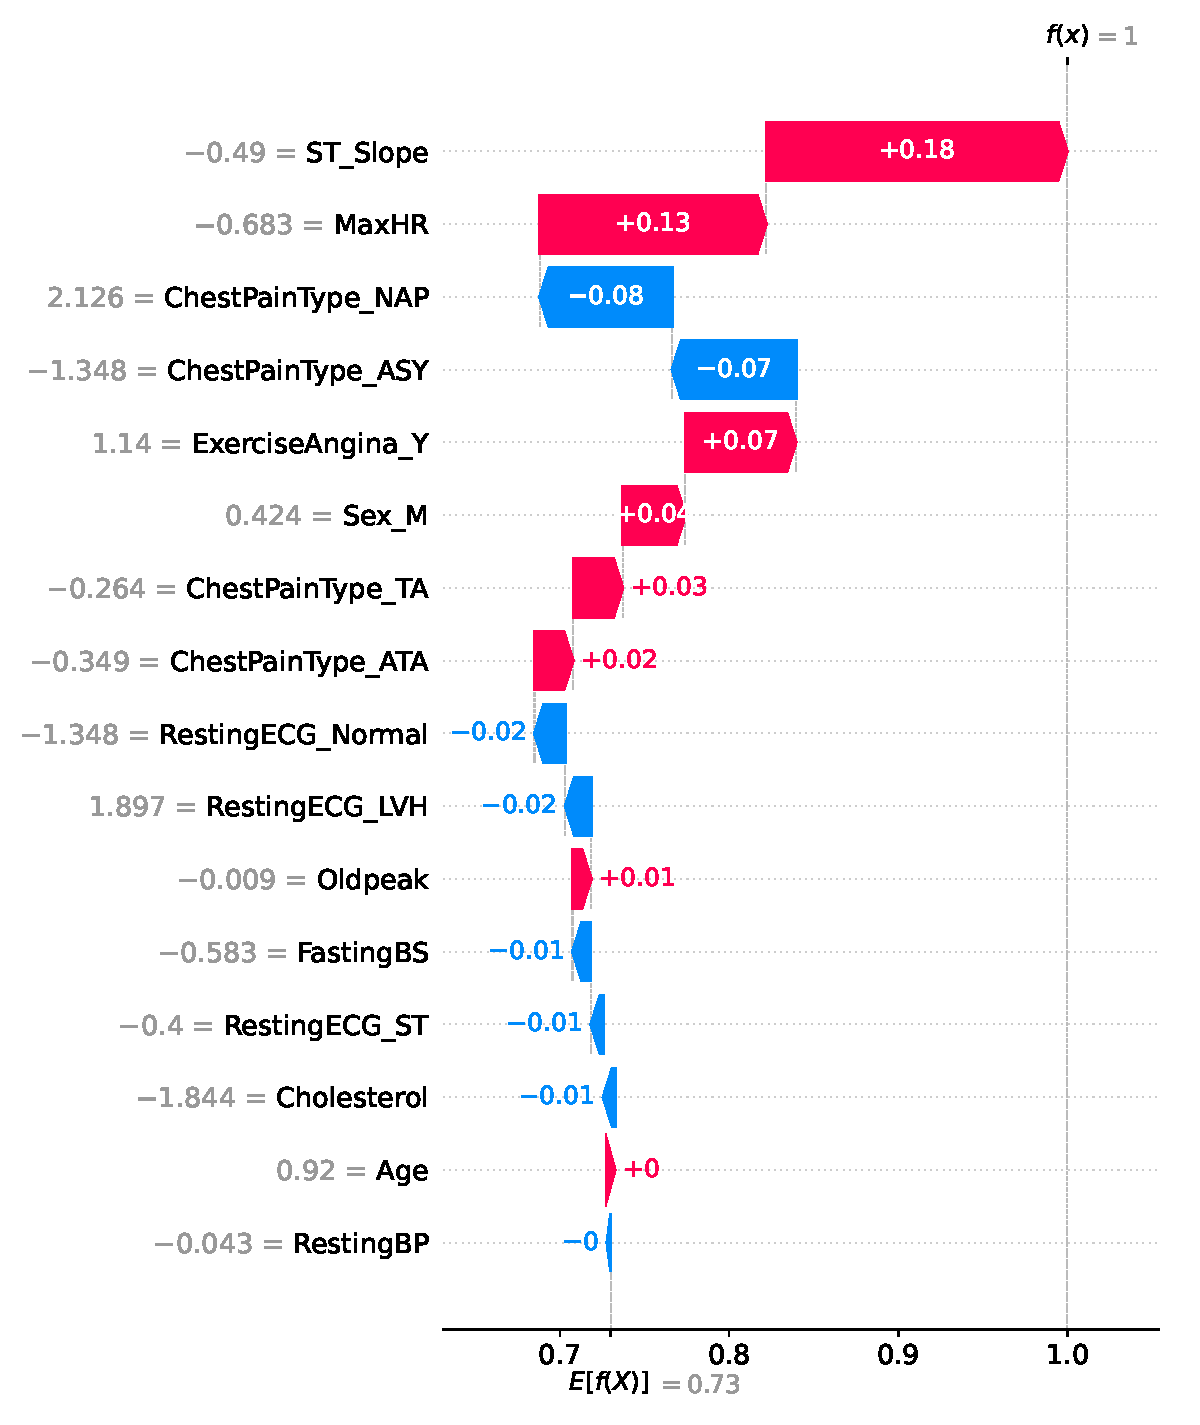
\includegraphics[width=1\textwidth]{images/shap_sample_positive_1.pdf}
        \caption{}
        \label{fig:shap_sample_positive_1}
    \end{subfigure}
    \begin{subfigure}{1\columnwidth}
        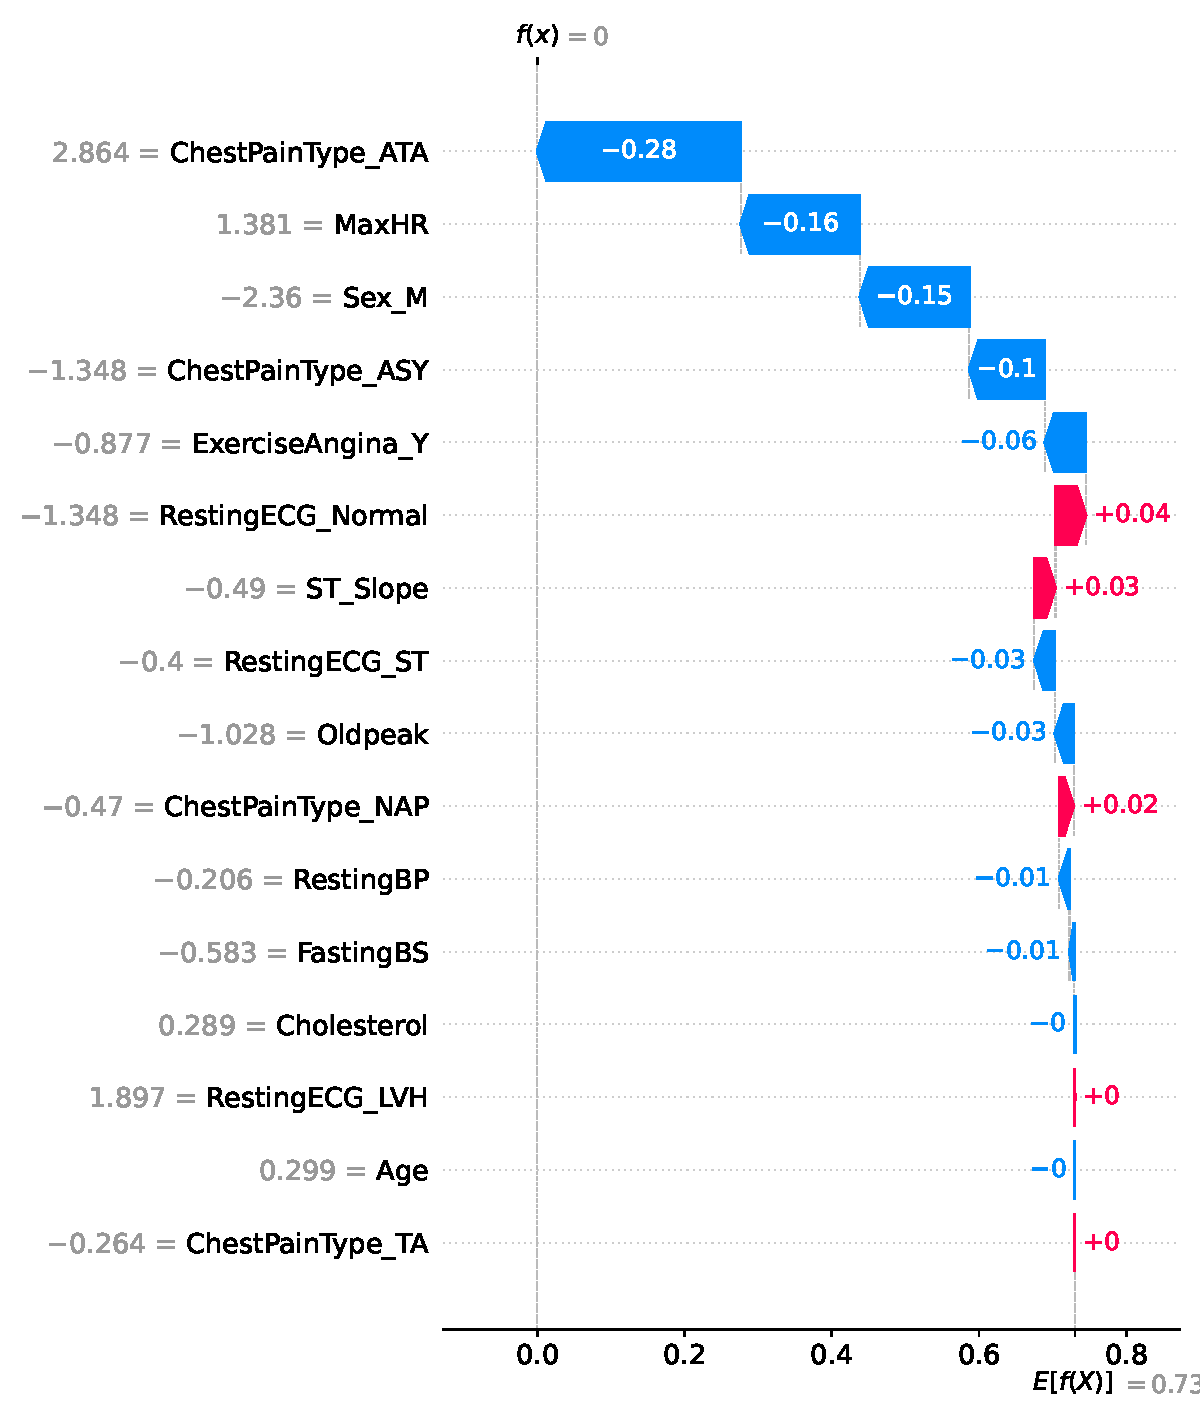
\includegraphics[width=1\textwidth]{images/shap_sample_positive_2.pdf}
        \caption{}
        \label{fig:shap_sample_positive_2}
    \end{subfigure}
    \begin{subfigure}{1\columnwidth}
        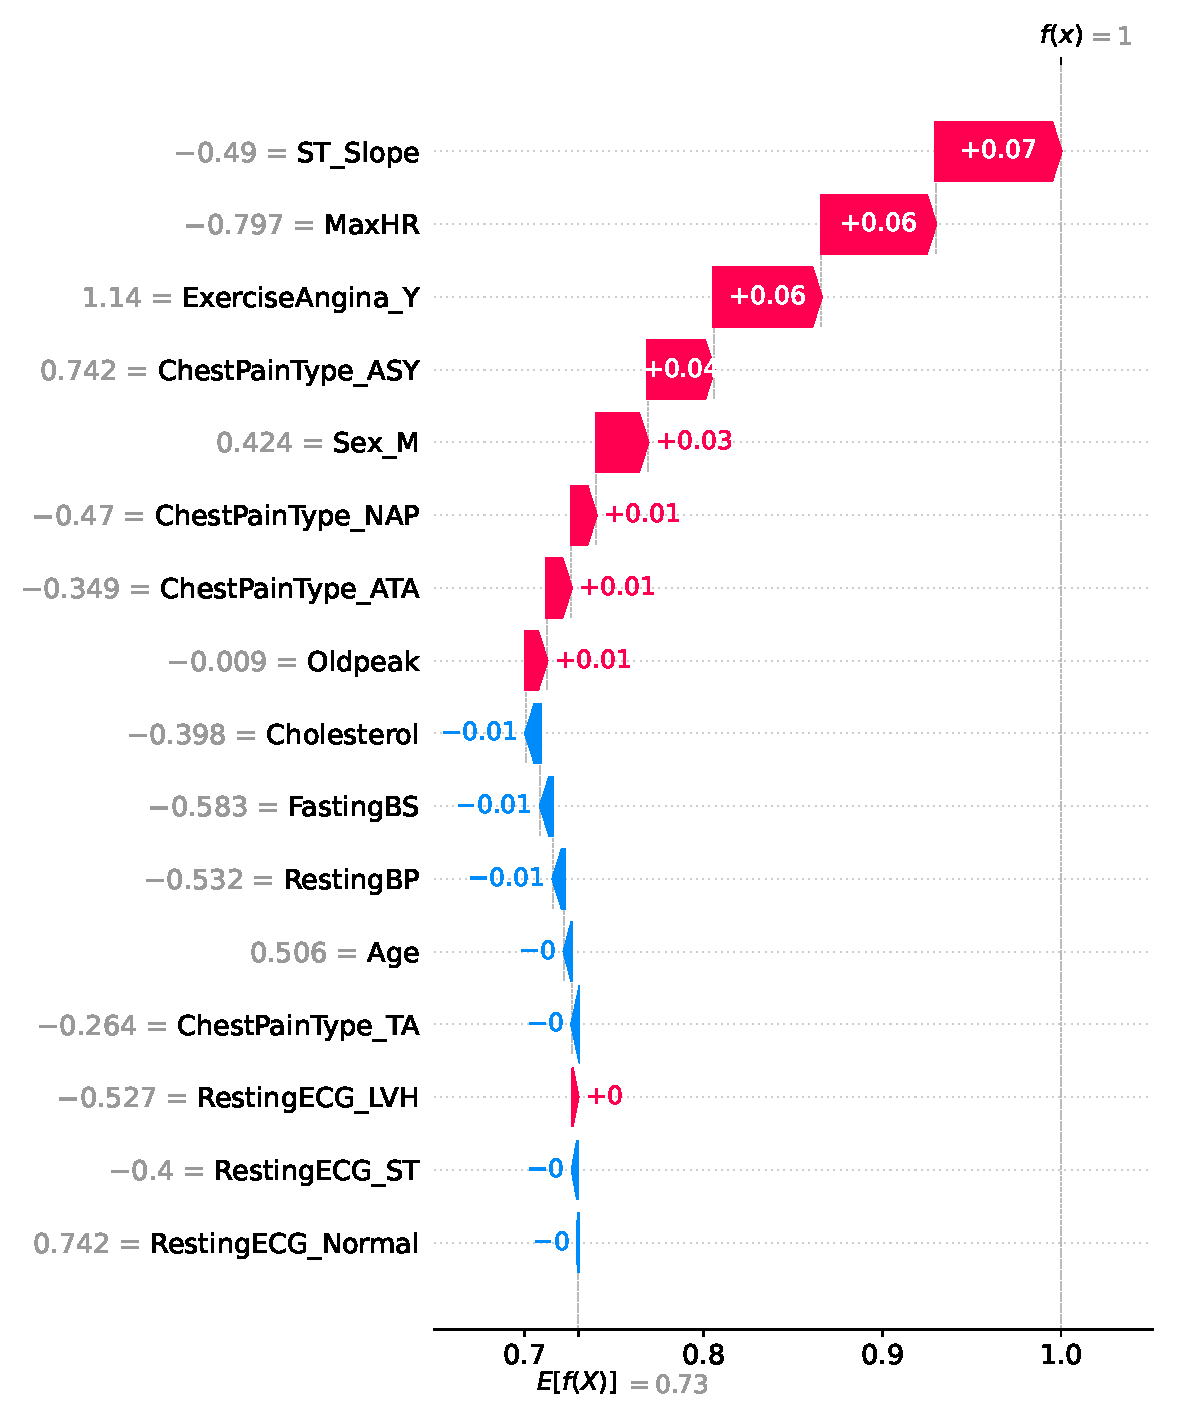
\includegraphics[width=1\textwidth]{images/shap_sample_positive_3.pdf}
        \caption{}
    \end{subfigure}
    \begin{subfigure}{1\columnwidth}
        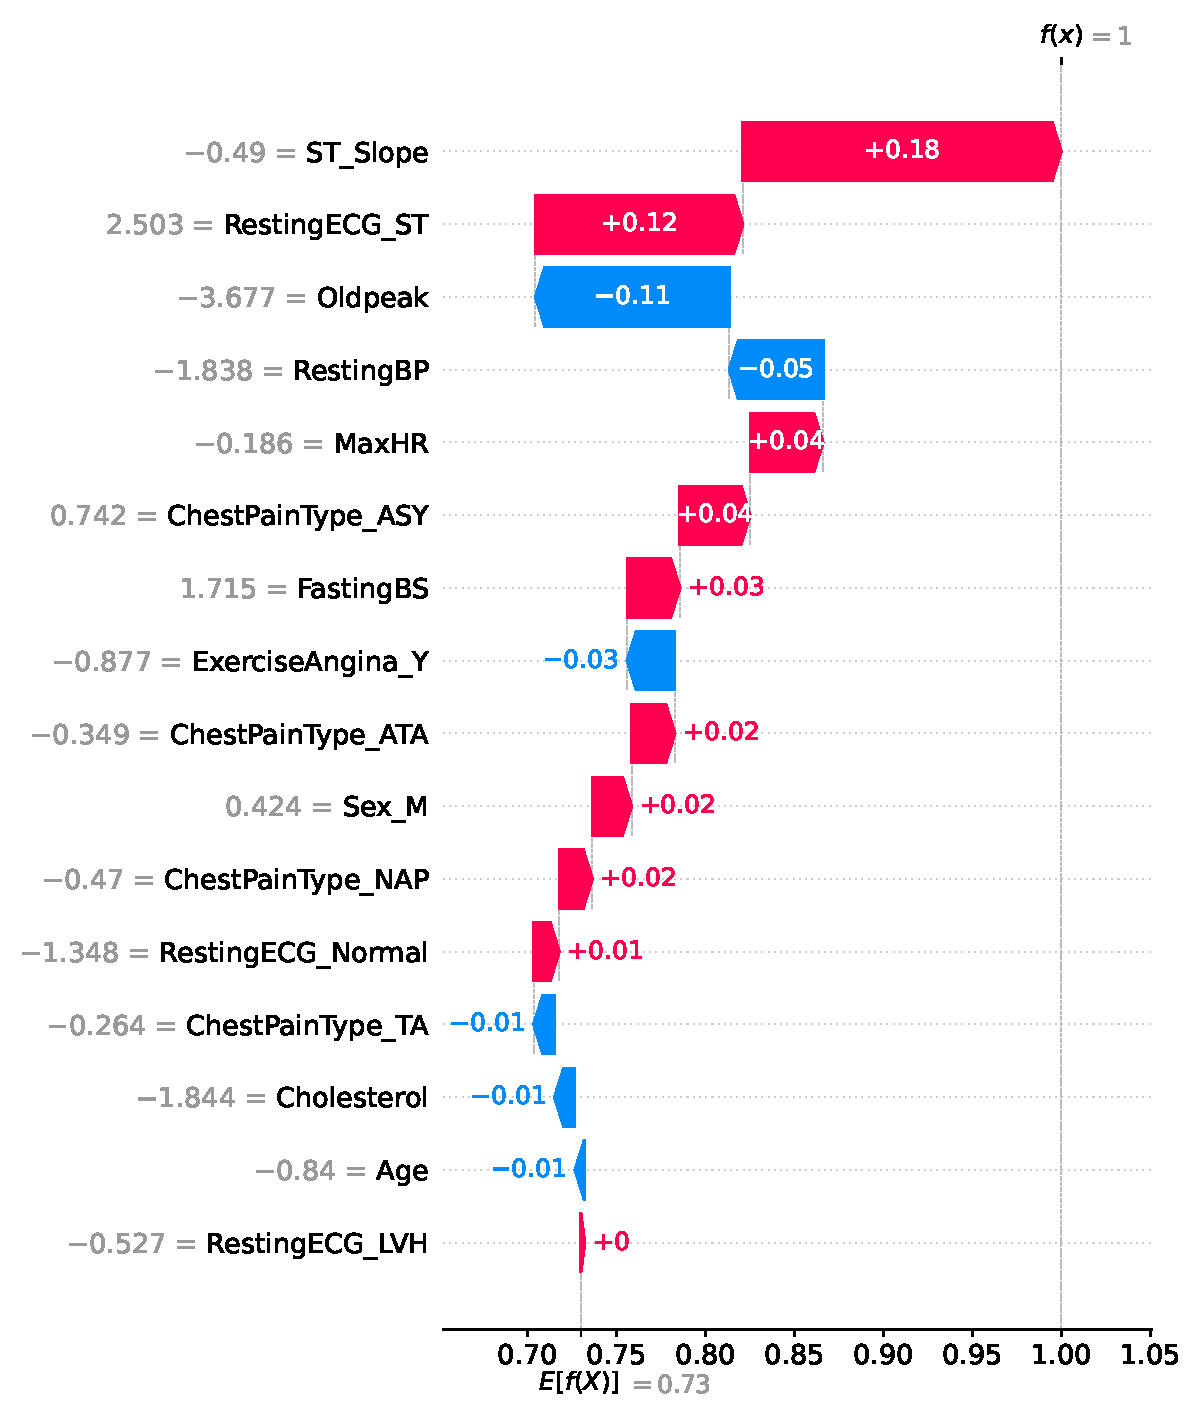
\includegraphics[width=1\textwidth]{images/shap_sample_positive_4.pdf}
        \caption{}
    \end{subfigure}
    \caption{Vizualization of SHAP explanations of the output of four \textbf{positive} samples from the test dataset. Features were normalized prior to calculating the Shapley values, as reflected in the displayed values of the samples. Note that sample in \protect\subref{fig:shap_sample_positive_2} has been misclassified as negative.}
    \label{fig:shap_sample_positive}
\end{figure*}
\begin{figure*}
    \centering
    \begin{subfigure}{1\columnwidth}
        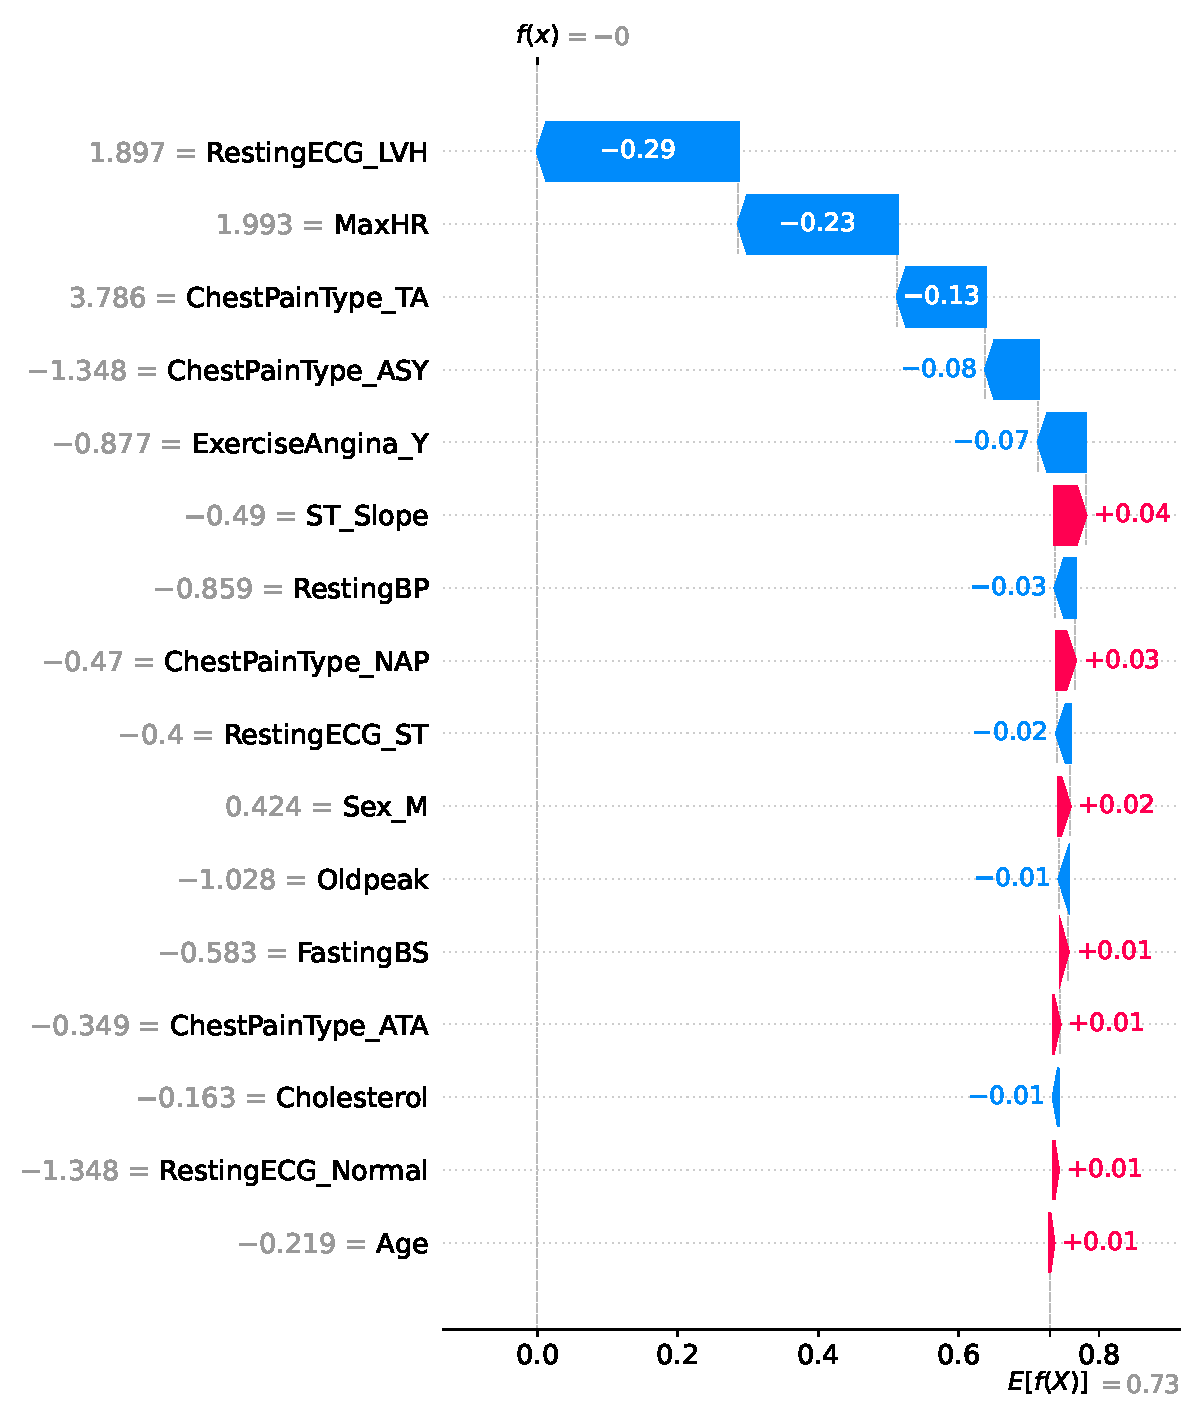
\includegraphics[width=1\textwidth]{images/shap_sample_negative_1.pdf}
        \caption{}
    \end{subfigure}
    \begin{subfigure}{1\columnwidth}
        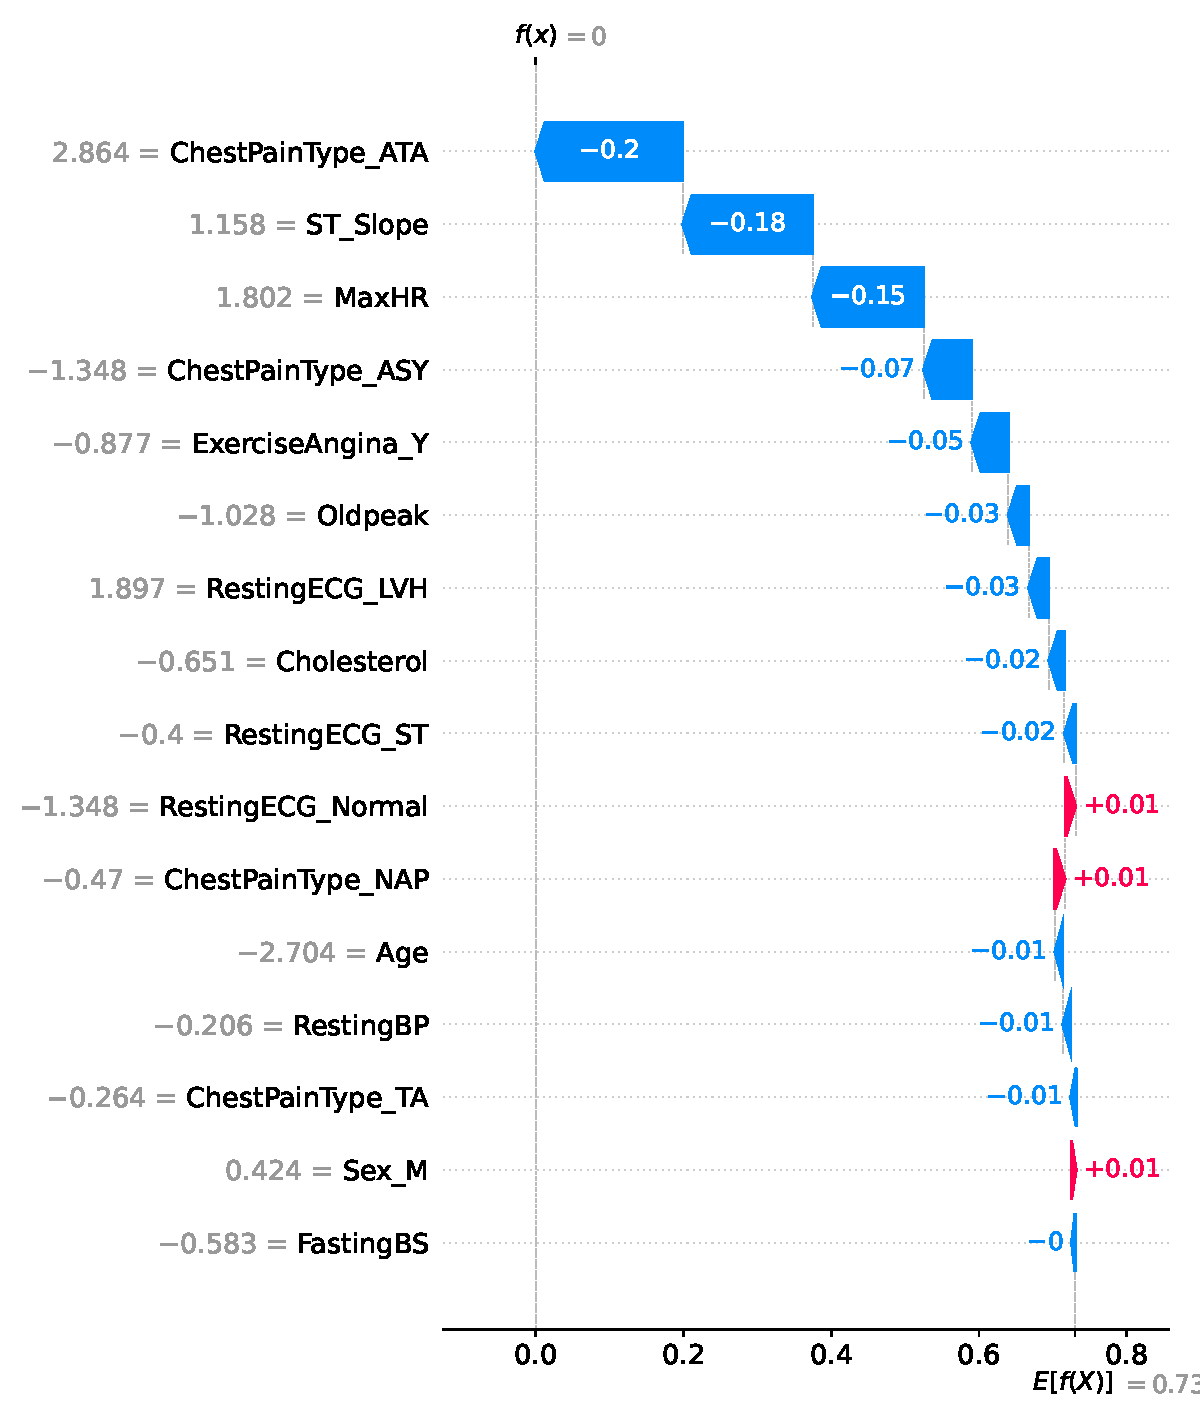
\includegraphics[width=1\textwidth]{images/shap_sample_negative_2.pdf}
        \caption{}
    \end{subfigure}
    \begin{subfigure}{1\columnwidth}
        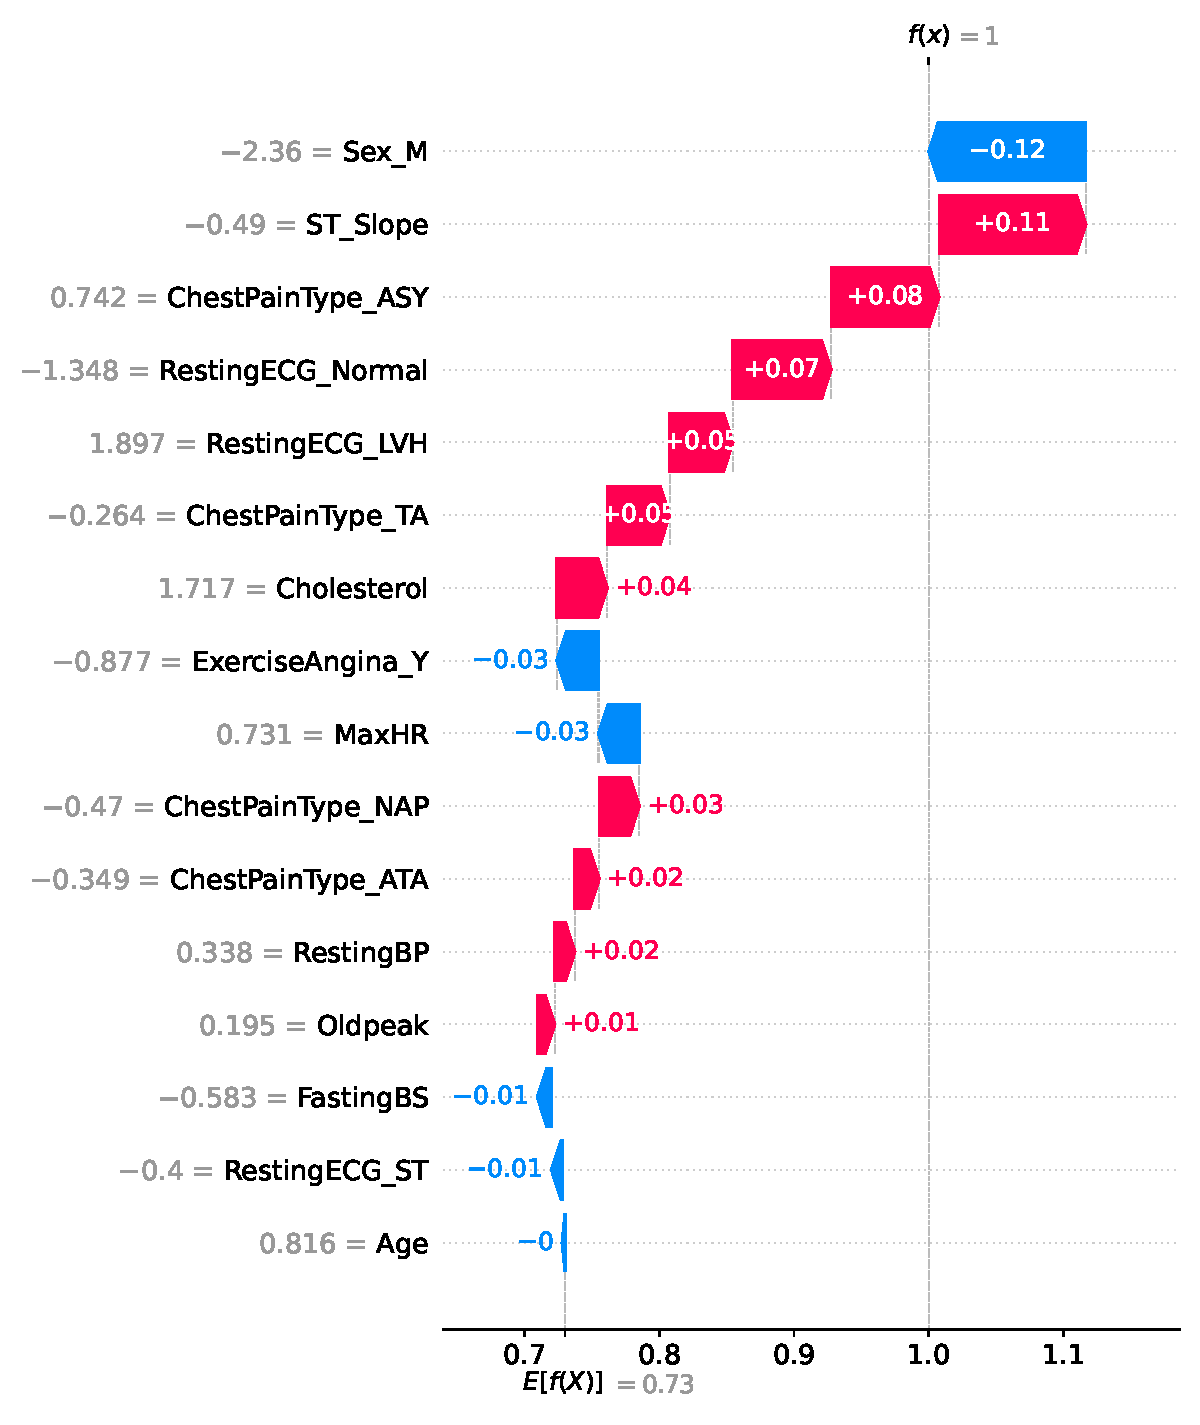
\includegraphics[width=1\textwidth]{images/shap_sample_negative_3.pdf}
        \caption{}
        \label{fig:shap_sample_negative_3}
    \end{subfigure}
    \begin{subfigure}{1\columnwidth}
        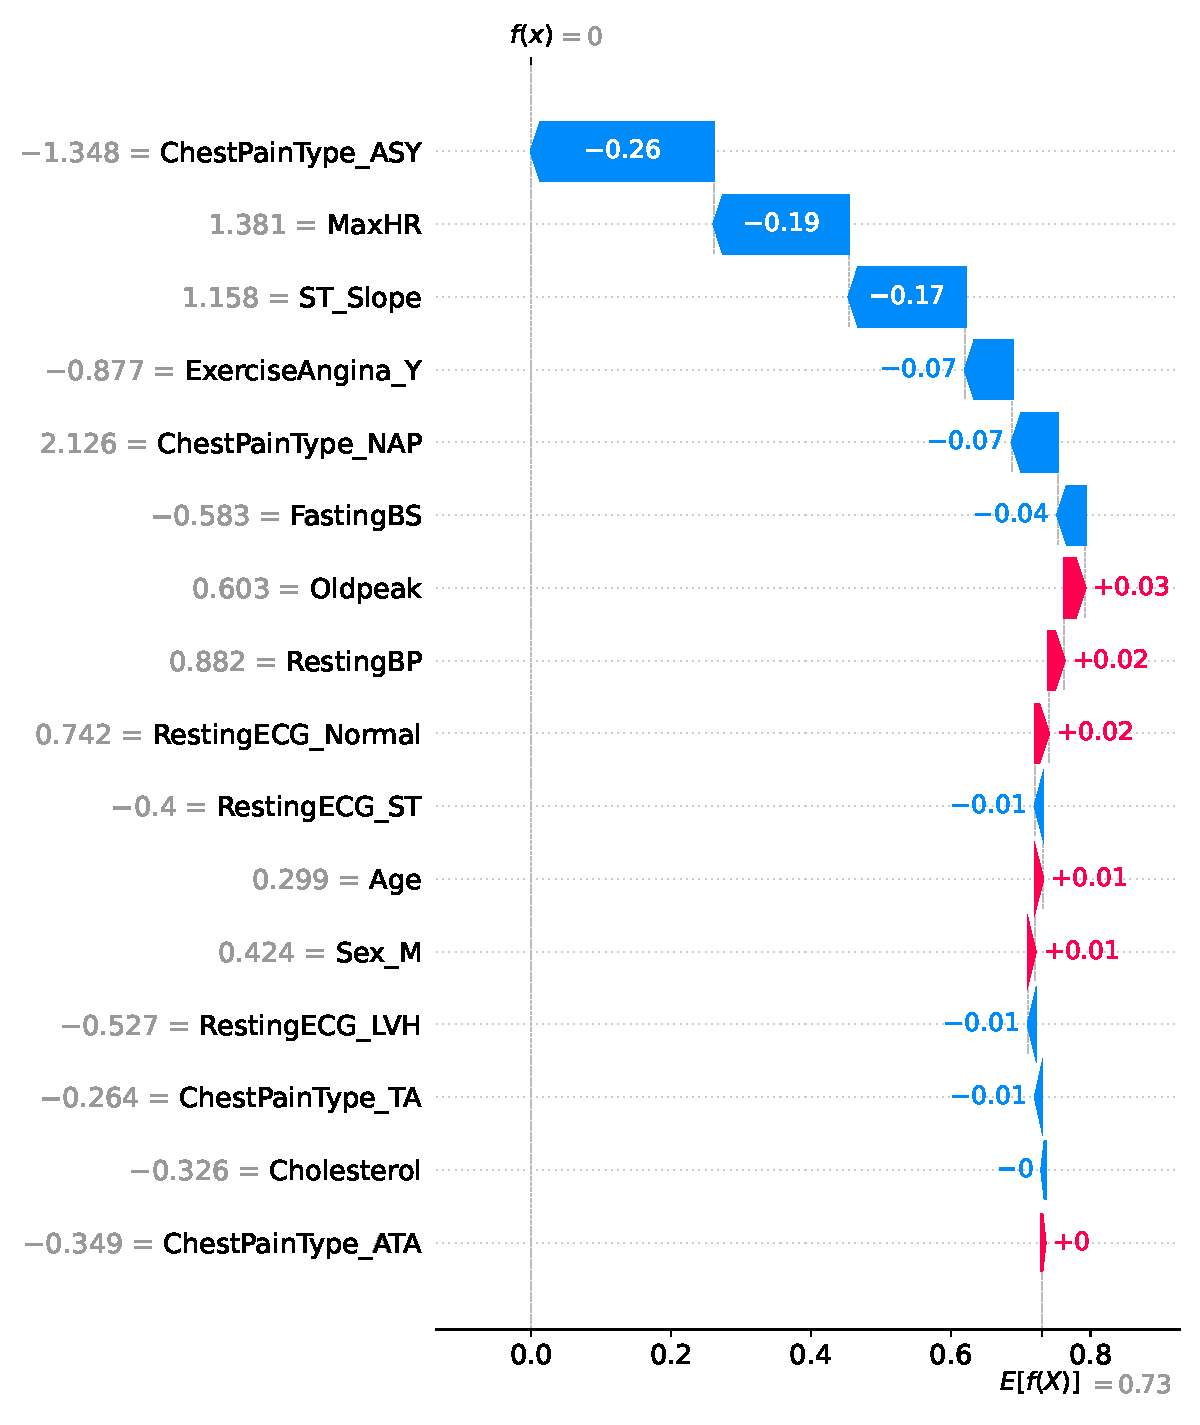
\includegraphics[width=1\textwidth]{images/shap_sample_negative_4.pdf}
        \caption{}
    \end{subfigure}
    \caption{Vizualization of SHAP explanations of the output of four \textbf{negative} samples from the test dataset. Features were normalized prior to calculating the Shapley values, as reflected in the displayed values of the samples. Note that the sample in \protect\subref{fig:shap_sample_negative_3} has been misclassified as positive.}
    \label{fig:shap_sample_negative}
\end{figure*}
